\section{Results}
\label{results}

All experiments were performed on VMware workstation 12 on live development server with the configuration Intel(R) Core (TM) i7-6500U CPU @ 2.50GHz, 30GB HDD, 2GB RAM for all virtual machines, and the operating system platform is Ubuntu 14.04.5 LTS Desktop 64-bit.

This section we divided into two part of evaluation: in first part we evaluate machine learning algorithm and its results for anomaly detection by Intrusion detection system and in the next part we focused on actual production and its results with snort experiment and attack detection and its respond. As summarized the java application converts decision tree into java program by taking J48 tree and the classified tree looks like Figure \ref{fig:J48tree}. Table \ref{table:J48result} and Figure \ref{fig:sum-roc} show the accurecy results of J48 algorithm and ROC curve for each type of traffic respectively.

\begin{table*}
\begin{center}
\begin{tabular}[width=\textwidth]{llllllllll}
\multicolumn{10}{l}{\bfseries === Detailed Accuracy By Class ===}\\
\\
 & TP Rate & FP Rate & Precision & Recall & F-Measure & MCC & ROC Area & PRC Area & Class\\
 & 0.996 & 0.033 & 0.994 & 0.996 & 0.995 & 0.967 & 0.987 & 0.995 & NORMAL\\
 & 0.976 & 0.003 & 0.981 & 0.976 & 0.979 & 0.975 & 0.991 & 0.977 & Probe\\
 & 0.820 & 0.001 & 0.890 & 0.820 & 0.854 & 0.853 & 0.957 & 0.777 & R2L\\
 & 0.934 & 0.000 & 0.959 & 0.934 & 0.947 & 0.946 & 0.980 & 0.950 & DoS\\
 Weighted Avg. & 0.991 & 0.029 & 0.991 & 0.991 & 0.991 & 0.967 & 0.987 & 0.990 & \\
\end{tabular}
\end{center}
\caption{Accuracy Result of J48 algorithm (based on our dataset)}
\label{table:J48result}
\end{table*}

\begin{figure}[h!]
	\centering
	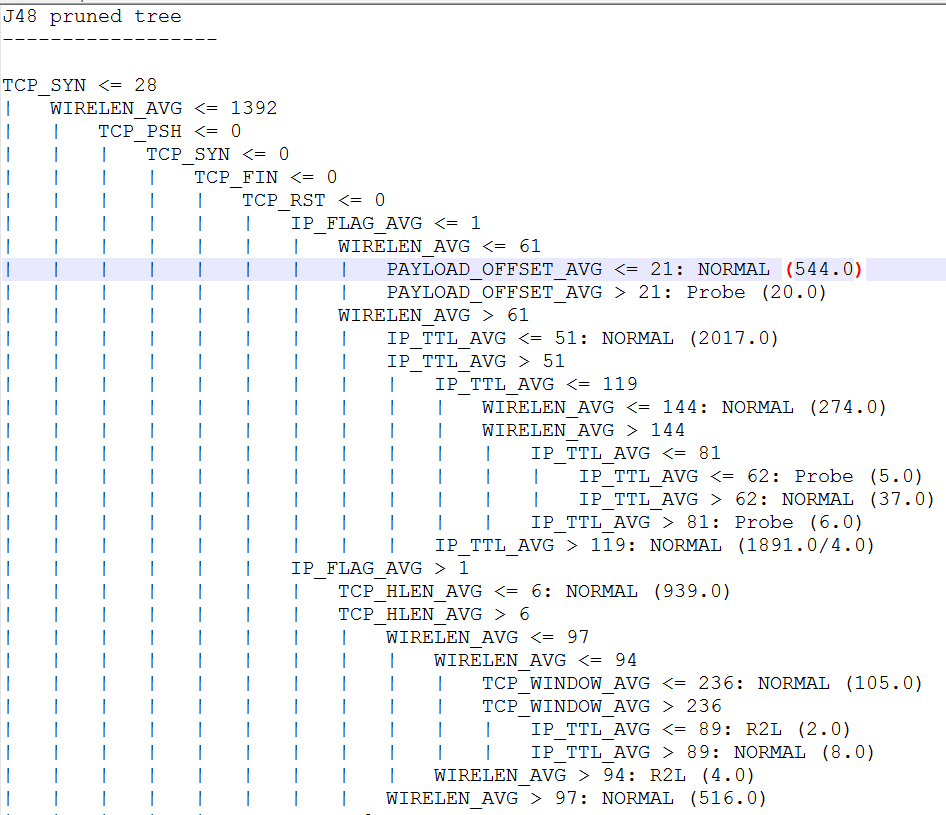
\includegraphics[width=\linewidth]{J48_tree.png}
	\caption{Sub part of pruned tree J48 Decision (based on our dataset)}
	\label{fig:J48tree}
\end{figure}

\begin{figure*}
	\centering
	\begin{subfigure}[t]{0.4\textwidth}
            \centering
            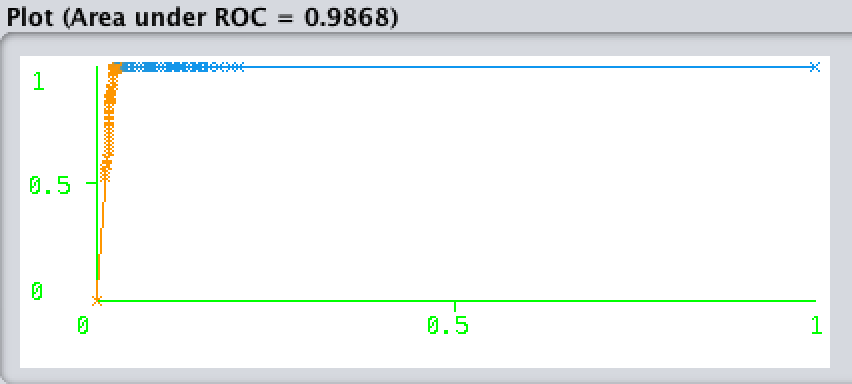
\includegraphics[width=\textwidth]{NORMAL.png}
            \caption{ROC-NORMAL}
            \label{fig:normal-roc}
        \end{subfigure}
        \quad
        \begin{subfigure}[t]{0.4\textwidth}
            \centering
            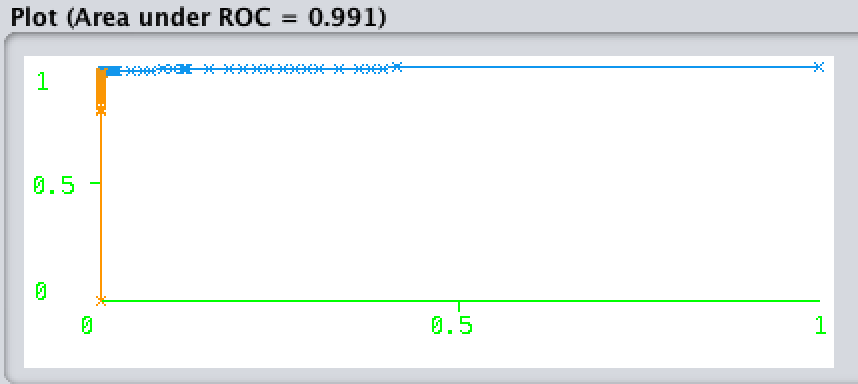
\includegraphics[width=\textwidth]{ProbeAttack.png}
            \caption {ROC-Probe}
            \label{fig:probe-roc}
        \end{subfigure}
        \vskip\baselineskip
        \begin{subfigure}[t]{0.4\textwidth}
            \centering
            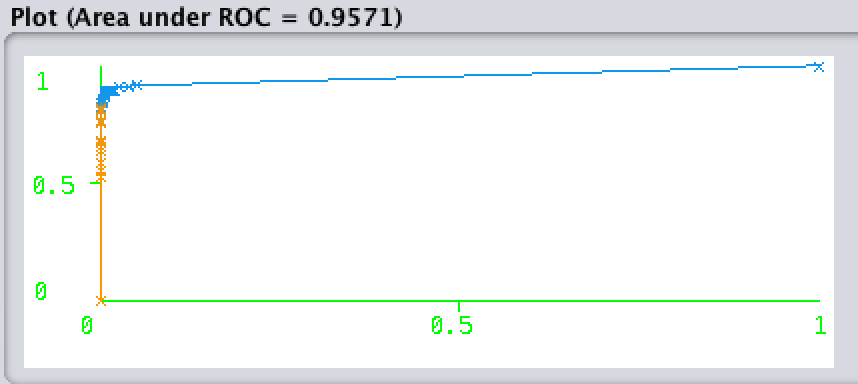
\includegraphics[width=\textwidth]{R2L.png}
            \caption{ROC-R2L}
            \label{fig:r2l-roc}
        \end{subfigure}
        \quad
        \begin{subfigure}[t]{0.4\textwidth}
            \centering
            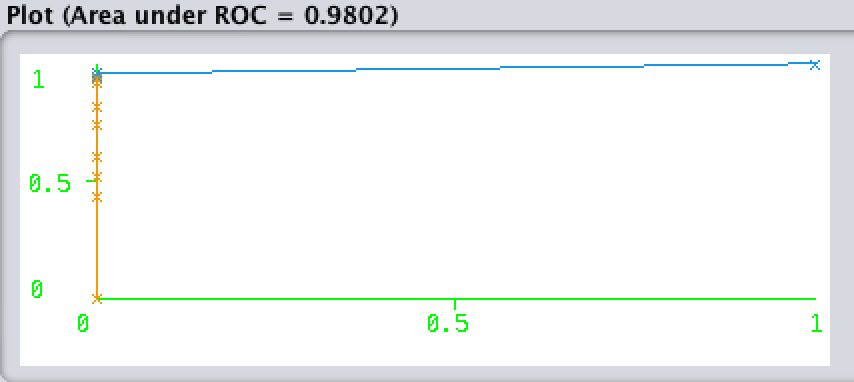
\includegraphics[width=\textwidth]{DoS.png}
            \caption{ROC-DoS}
            \label{fig:dos-roc}
        \end{subfigure}
        \caption{The ROC Curves for each type of traffic}
        \label{fig:sum-roc}
\end{figure*}

In second part, by evaluating snort system which generates snort rule and push them into existing snort configuration and restart snort service. Finally we got a whole working machine which works on J48 machine learning algorithm for detecting intrusion and generating snort rule in real-time and restart snort service with any packet loss. If it detects any attempt to exploit machine can respond by itself by dropping all incoming packets coming from attacker's IP. We uses one common rule for DOS and DDOS detection so machine can detect both of them but can't mitigate DDOS attack though it can detect successfully.

In accuracy results, ROC- space shows area under the curve (AUC) is 98\% of accurate for Normal traffic. It classified Probe, R2L, Dos attacks with 99\%, 95\% and 98\% accurate results respectively. Here, ROC Curves can be used to evaluate the tradeoff between TP (true-positive) and FP (false-positive) rates of classification algorithm. We got some false prediction in which actual attack predicted as normal and same as some normal pattern classified as an attack and got some false alarm by the machine learning classifier. Dos results shows that there is 0.0 FP rate with the classification algorithms.
